%!TEX root = thesis.tex

\chapter{Methodology}
\label{chapter:methodology}


%TODO explain methodology to obtain results of quantum clustering of just present results on why it wasn't viable?

%TODO This is where I explain my approach to the problem of EAC in Big Data

The aim of this thesis is the optimization and scalability of EAC, with a focus for large datasets. EAC is divided in three steps and each has to be considered for optimization.

The first step is the accumulation of evidence, i.e. generating an ensemble of partitions. The main objective for the optimization of this step is speed. Using fast clustering methods for generating partitions is an obvious solution, as is the optimization of particular algorithms aiming for the same objective. Since each partition is independent from every other partition, parallel computing over a cluster of computing units would result in a fast ensemble generation. Using either or any combination of these strategies will guarantee a speedup.


	
The second step is mostly bound by memory. The complete co-association matrix has a space complexity of $\mathcal{O}(n^2)$. Such complexity becomes prohibitive for big data, e.g. a dataset of $2 \times 10^6$ samples will result in a complete co-association matrix of $14901 \; GB$ if values are stored in single floating-point precision.

The last step has to take into account both memory and speed requirements. The final clustering must be able to produce good results, fast while not exploding the already big space complexity from the co-association matrix.

Initial research was under the field of quantum clustering. After this pursuit proved fruitless regarding one of the main requirements (computational speed), the focus of researched shifted to parallel computing, more specifically GPGPU. 

\section{Quantum Clustering}

Research under this paradigm aimed to find a solution for the first and last steps. Two venues were explored: Quantum K-Means and Horn and Gottlieb's quantum clustering algorithm.
For both, the experiments that were setup had the goal of evaluating the speed and accuracy performances of the algorithms.

Under the qubit concept, no other algorithms were experimented with since the results for this particular algorithm showed that this kind of approach is infeasible due to the cost in computational speed. The results highlight that fact.



\section{Speeding up Ensemble Generations with Parallel K-Means}
K-Means is an obvious candidate for the generation of partitions since it is simple, fast and partitions don't require big accuracy - variability in the partitions is a desirable property which translates in few iterations. For that reason, optimizing this algorithm ensures that the accumulation of evidence is performed in an efficient manner.
Furthermore, it is not necessary for K-Means to produce accurate clusterings, e.g. K-Means doesn't have to converge - 3 iterations should suffice. The reason for this is the desire for variability within the partition population.


%TODO pseudocode & diagrams
%TODO explain the solution for GPGPU K-Means

\section{Dealing with space complexity of coassocs}

\subsection{Exploiting the sparsity of the co-association matrix}



Which method is more effective in very large datasets, however, would depend on the dataset. The sparsity maximization approach got very low densities for some datasets, close to $0.01$ in some cases. This is already a big improvement

Either way, the CSR data structure is used to store the co-association matrix. 
Due to the sparse nature of the co-association matrix, storing it n this format can decrease used space to as much as $10\%$, depending on the sparsity of the matrix as shown in \cite{Lourenco2010}. 
This is also an important step since the co-association matrix is already in the correct format for the computation of the final clustering within the GPGPU paradigm.

\subsection{Using prototypes}

\subsubsection{k-Nearest Neighbors as prototypes}
In the literature review, another approach to reduce the complexity of the co-association matrix is to use the $p$ closest neighbors of each sample. Previous to building the co-association matrix, the $p$ closest samples to each sample are computed and stored in the $n \times p$ neighbor matrix. The co-association matrix is reduced to size $n \times p$ and only considers the neighbors of each sample during the voting mechanism. This means two $n \times p$ matrices have to be stored, which, as long as $p$ is significantly lowers than the number of samples, is close to a sparse representation of the full matrix.

It would be ideal to combine both approaches (sparsity and neighbors) to further reduce space complexity, but they're not necessarily compatible. When the neighbor approach is used, it is unlikely that a sample will never be clustered with it's closest $p$ neighbors. However, this highly depends on the the number of neighbors relative to the number of samples and also the granularity of the partitions. If the number of neighbors is high, one of the neighbors can be sufficiently far away from the sample to not clustered with it. If the granularity of the partitions is high (i.e. there are a high number of small clusters) then each cluster may have sufficiently few samples that neighbors are not included. This means that the $n \times p$ co-association matrix may not have many zeros which translates in little return for using the sparsity augmentation approach. To illustrate this point, let's consider a dataset of $10^6$ patterns. 

%comment on which method is more effective, maybe some experiment is needed to see which
%demonstrate why both methods are not compatible - a simple filling of knn matrix should suffice

\subsubsection{Random prototypes}
A second prototype approach is to choose $p$ random non-repetitive samples as prototypes. This will be the same for every sample.
Here the voting mechanism is altered so that if a sample is clustered with any of the prototypes, the correspondent element in the co-association matrix is incremented. This has the advantage that only a $n \times p$ matrix needs to be stored along with a $p$ array for the prototypes.
Furthermore, if $p$ if high enough to provide a representative sample of the dataset the results can be as good as the full matrix

\subsubsection{Medoid prototypes}
This approach is similar to the random prototypes but, instead of choosing $p$ random samples from the dataset, the prototypes will be the representatives of the dataset from another algorithm, e.g. K-Medoids, K-Means.

\section{Hierarchical Agglomerative Clustering step}

\subsection{HAC and GPGPU}
% introduction to the procedure of SL with MST
Since SL-HAC is an inherently sequential algorithm, an efficient GPU version is hard to implement.
However, SL-HAC can be performed by computing the MST and cutting edges until we have the desired number of clusters.
Considerable speedups are reported in the literature for MST solvers in the GPGPU paradigm.
The considered solution uses the efficient parallel variant of Borůvka's algorithm \cite{Sousa2015}. 
If the number of clusters is given the necessary cuttings are done on the MST. 
If not, the number of clusters is computed with the lifetime technique. 
A new graph in the CSR format is computed from the altered MST and is then fed to the labelling algorithm, which will provide the final clustering.

\subsubsection{Generating the MST}
% explain modification to the MST algorithm to accept unconnected graphs
The output of the Borůvka's algorithm is a list of the indices of the edges constituting the MST. 
These indices point to the \emph{destination} of the original graph. 
The original algorithm in \cite{Sousa2015} assumes fully connected graphs, but this is not guaranteed in the EAC paradigm.
In graph theory, given a connected graph $G = (V,E)$, there is a path between any $s,t \in V$.
In an unconnected graph, this is not the case and unconnected subsets are called components, i.e. a connected component $C \subset V$ ensures that for each $u,v \in C$ there is a path between $u$ and $v$.
In the present implementation, the issue of unconnected graphs was solved in the first step (finding the minimum edge connected to each vertex or supervertex). 
If a vertex has no edges connected to it (an outdegree of 0 since all edges are duplicated to cover both directions) then it is marked as a mirrored edge. 
This means that the independent components will be marked as supervertices in all subsequent iterations of the algorithm. 
The overhead of having this unnecessary vertices is low since the number of independent components is typically low compared to the number of vertices in the the graph and since the processing of such vertices is very fast.
As a consequence, the stopping criteria becomes the lack of edges connected to the remaining vertices, which is the same as saying that all elements of the \emph{outdegree} array are zero. 
This condition can be checked as a secondary result of the computation of the new \emph{first\_edge} array. 
This step is performed by applying an exclusive prefix sum over the \emph{outdegree}. 
The prefix sum was implemented in such a way that it returns the sum of all elements, which translates in very low overhead to check this condition.
The final output is the MST array and the number of edges in the array. 
The later is necessary because the number of edges will be less than $|V|-1$ when independent components exist, and also because the MST array is pre-allocated in the beginning of the algorithm when the number of edges is not yet known.

\subsubsection{Number of clusters and cutting edges}
% cutting edges
The number of clusters can be automatically computed with the lifetime technique or be supplied. 
Either way, a list (\emph{mst\_weights}) with the weights of each edge of the MST is compiled and ordered.
The list of edges is also ordered according to the order of the \emph{mst\_weights}. 
If the number of clusters $k$ was given, the algorithm removes the $k - 1$ heaviest edges. 
If there are independent components inside the MST those are taken into consideration before removing any edges.
If the number of clusters $k$ is higher than the number of independent components the final number of clusters will be the number of independent components.

To compute the number of clusters (which results in a truly unsupervised method) the lifetimes are computed.
In the traditional EAC, lifetimes are computed on the weights of the clusters by the order they're formed.
With the MST, the lifetimes are computed over the ordered \emph{mst\_weights} array, which is equivalent.
If there are independent components, an extra lifetime that will serve as the threshold between choosing the number of independent components as the number of clusters or looking into the lifetimes within the MST.
This is because links between independent vertices are not included in the MST.
For this reason, the lifetime for going from independent edges to the heaviest link in the MST (where the first cut would be performed) is computed separately.
If the maximum lifetime within the MST is bigger than the threshold, than the number of clusters is computed as in traditional EAC plus the number of independent components.
Otherwise, the independent components will be the final clusters.
Most of this process can be done by the GPU.
Library kernels were used to sort the array and compute the $arg max$, and a simple kernel was used to compute the lifetimes.

\subsubsection{Building the new graph}
The final MST (after performing the edge cuts, if any) is then converted into a new, reduced graph.
The function responsible for this takes the original graph and the final selection of edges contituting the MST and, afterwards, produces a graph in CSR format.
The function has to count the number of edges for each vertex, compute the origin vertex of each edge (the original \emph{destination} array only contains the destination vertices) and, with that information, build the final graph.
This process can be done by the GPU with simple mapping kernels.

\subsubsection{Final clustering}
The last step is computing the final clusters.
Any cut in the MST translates in independent components in the constructed graph.
This means that the problem of computing the clusters translates into a problem of finding independent connected components in a graph, a problem that usually goes by the name of Connected Component Labeling.
To implement this part in the GPU, the aforementioned Borůvka algorithm was modified to output the an array \emph{labels} of length $|V|$ such that the $i-th$ position contained the label of the $i-th$ vertex.
To this effect, the flow of the algorithm was slightly altered as shown in Figure \ref{fig:connected comps flow}. 
The kernel dealing with the MST was removed and a kernel to update the labels at each iteration, shown in Algorithm \ref{alg:comp_labels}, was implemented.
In the first iteration of the algorithm the converged colors are copied to the labels array.
In every iteration the kernel to update the labels takes in the propagated colors and the array with the new vertex IDs.
For each vertex in the array, the kernel first takes in the the color of the current vertex and maps it to the new color (remember that the color is actually a vertex ID and that that vertex has had its color updated).
Afterwards, the kernel maps the new color with the new vertex ID that color will take, to keep consistency with future iterations.

\begin{figure}[hbtp]
\centering
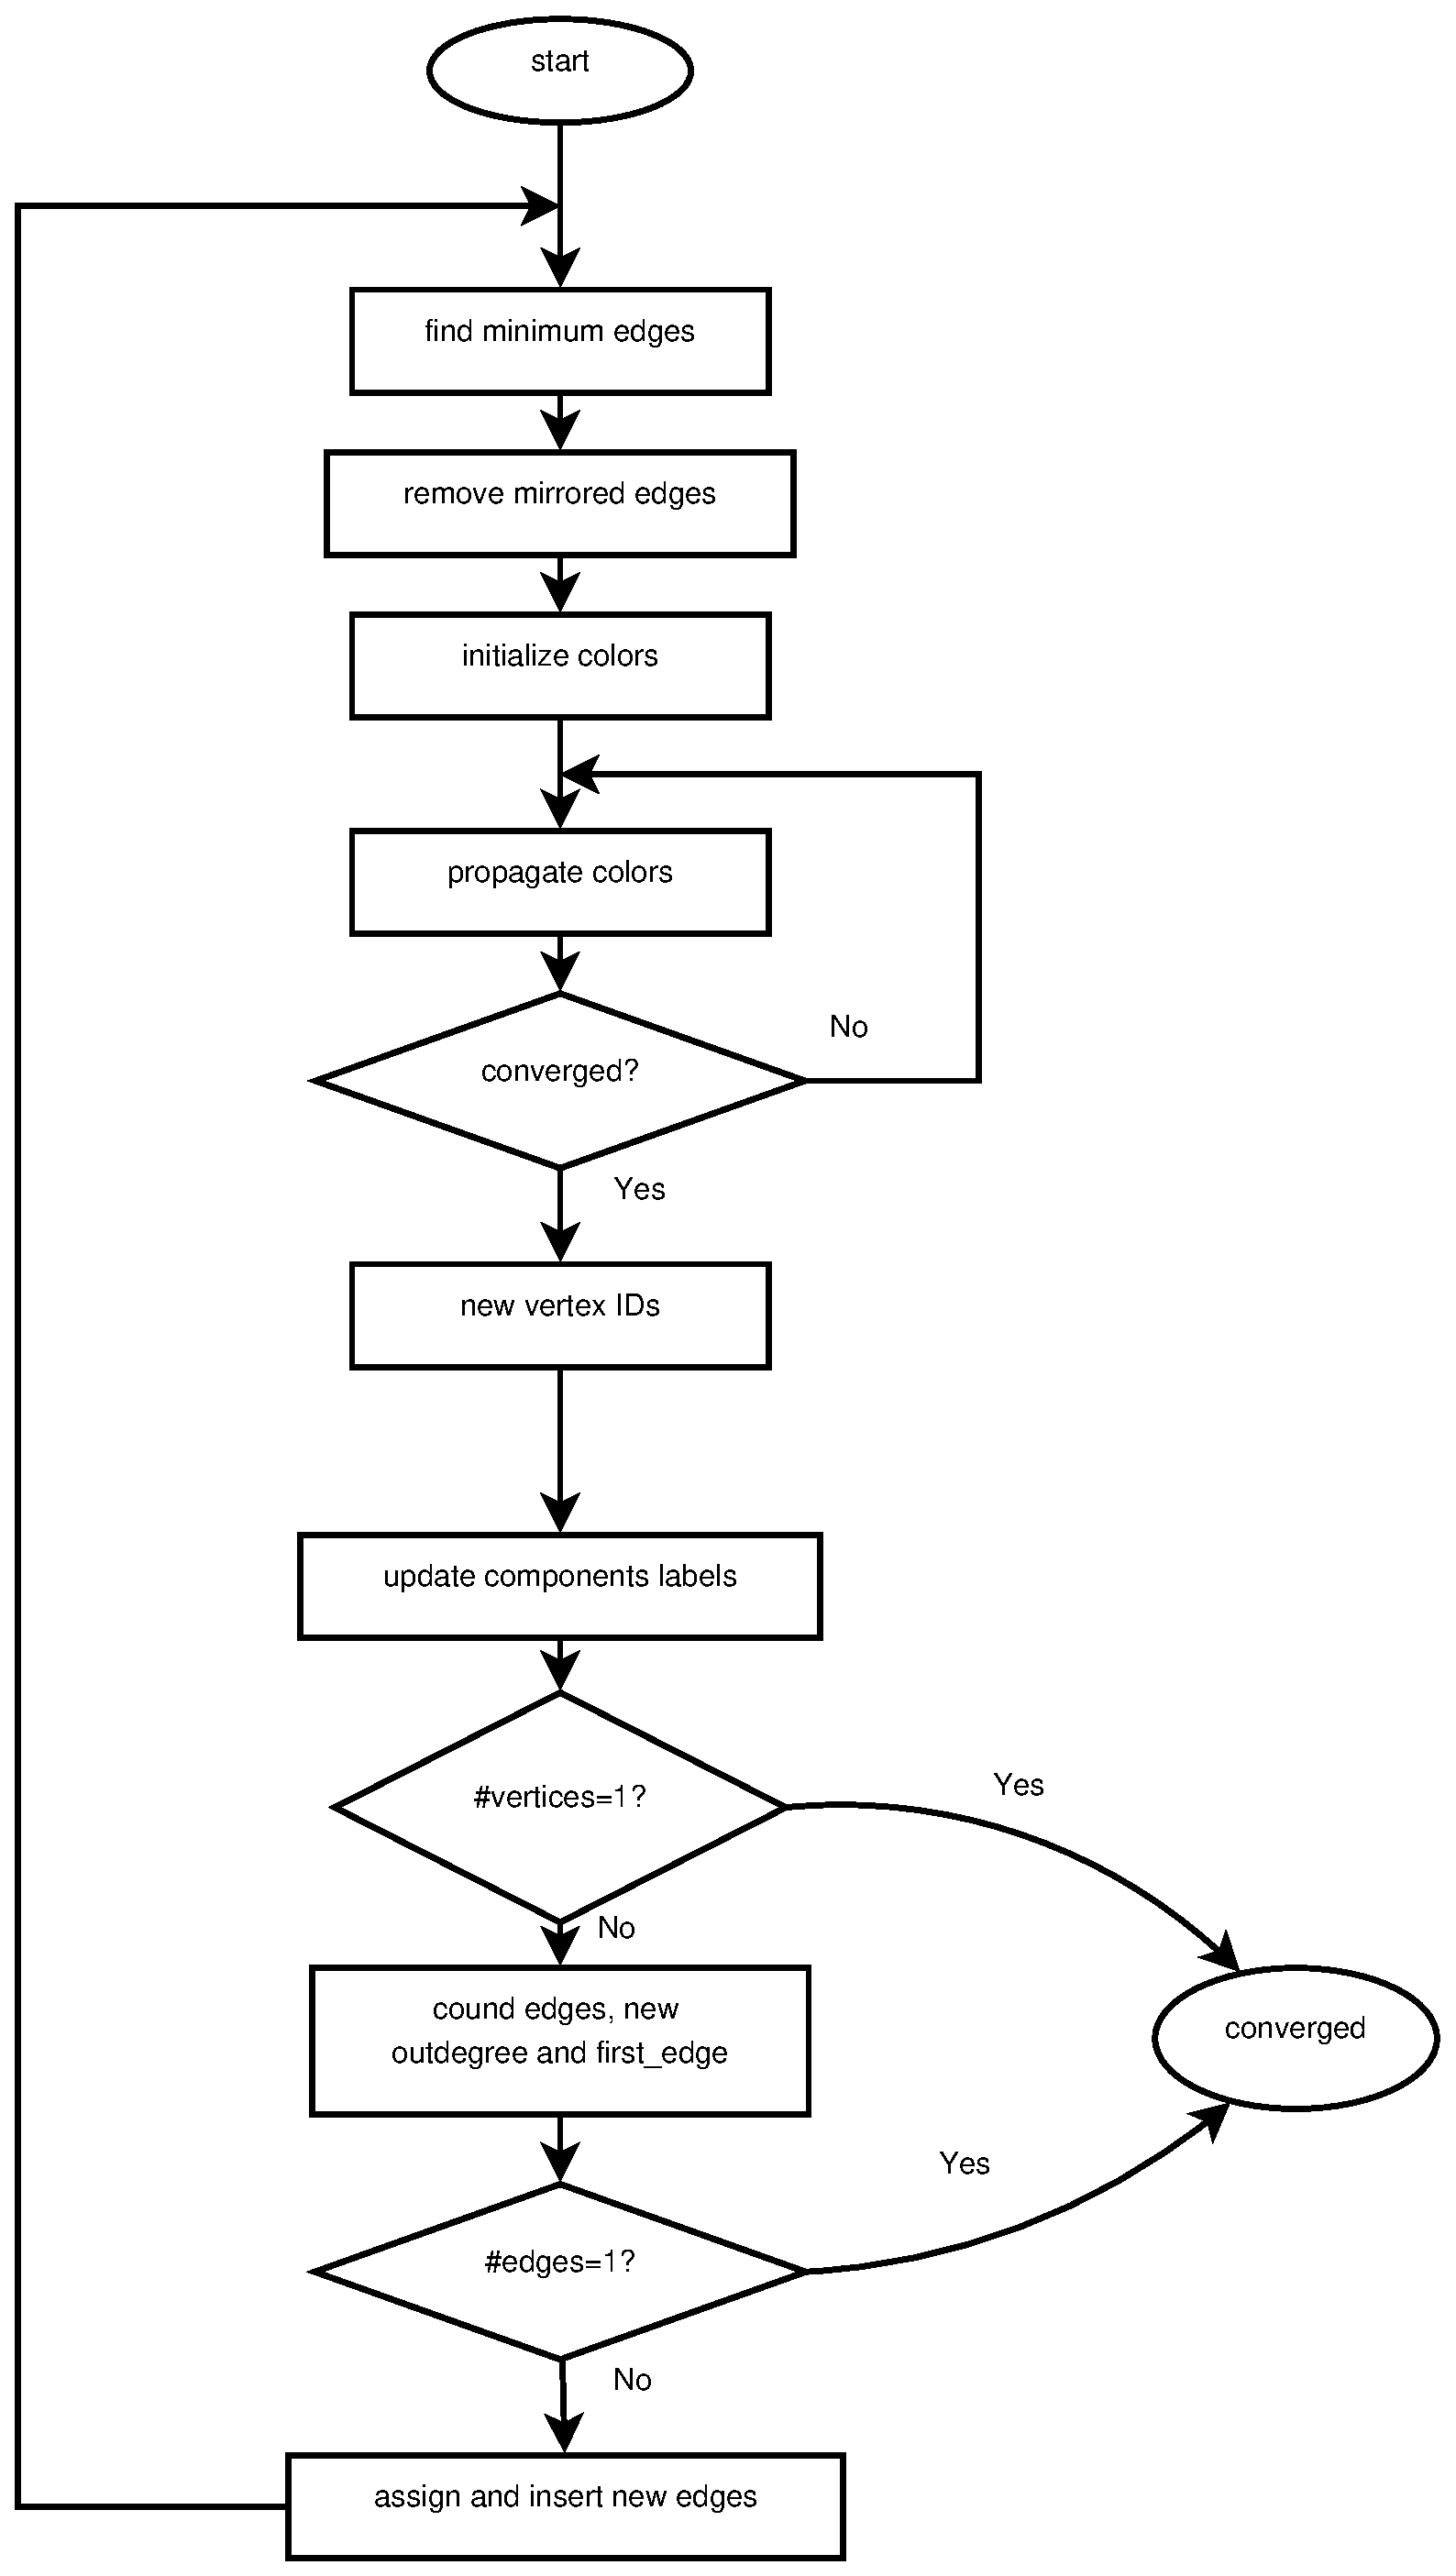
\includegraphics[scale=0.5]{methodology/connected_components_boruvka_flow.eps}
\caption{Diagram of the connected components labeling algorithm used.}
\label{fig:connected comps flow}
\end{figure}


%
% describe connected components algorithm
% how it copies colors in the first time
% and then just updates the labels with the new vertex IDs
%
% put flowchart and pseudocode


\begin{algorithm}
\caption{Update component labels kernel}\label{alg:comp_labels}
\begin{algorithmic}[1]
\Procedure{update\_labels}{$vertex\_id, labels, colors, new\_vertex$}
\State $curr\_color \gets labels[vertex\_id]$
\State $new\_color \gets colors[curr\_color]$
\State $new\_color\_id \gets new_vertex[new\_color]$
\State $labels[vertex\_id] \gets new\_color\_id$
\EndProcedure
\end{algorithmic}
\end{algorithm}



\subsubsection{Memory transfer with the GPU}
The whole algorithm of computing the SL clustering has been implemented in the GPU with minimizing the memory utilization in mind.
Transferring the initial graph is the most relevant memory transfer.
It has to be transfered twice: first for computing the MST and then to build the processed MST graph.
This happens because the initial device arrays used for the graph are deallocated to give space for the arrays of subsequent iterations of the MST algorithm.
This implementation design had in mind memory consumption in mind and could easily be avoided with the cost of having to store the bigger initial graph for the entire duration of the MST computation, which might be worthwhile if the GPU memory is abundant.
The final labels array is transfered back to the host in the end of computation, but its size is small relative the to the size of the original graph.
Furthermore, because the control logic is processed by the host and it is dependent on some values computed by the device, extra memory transfers of single values (e.g. number of vertices and number of edges on each iteration) are necessary.
These, however, may be safely dismissed since they're of little consequence in the overall computation time.


\begin{tabular}{lrrr}
\toprule
% \hline
{} &  threshold &   max\_assocs &  nnz percent relative to max \\
\midrule
% \hline
0  &   0.000000 &  1228.000000 &                     0.979769 \\
1  &   0.050000 &   794.000000 &                     0.613603 \\
2  &   0.100000 &   597.000000 &                     0.471318 \\
3  &   0.150000 &   496.000000 &                     0.386988 \\
4  &   0.200000 &   437.000000 &                     0.325645 \\
5  &   0.250000 &   367.000000 &                     0.276588 \\
6  &   0.300000 &   335.000000 &                     0.235490 \\
7  &   0.350000 &   294.000000 &                     0.200629 \\
8  &   0.400000 &   262.000000 &                     0.170249 \\
9  &   0.450000 &   232.000000 &                     0.143376 \\
10 &   0.500000 &   205.000000 &                     0.119374 \\
11 &   0.550000 &   167.000000 &                     0.098120 \\
12 &   0.600000 &   142.000000 &                     0.079426 \\
13 &   0.650000 &   121.000000 &                     0.062757 \\
14 &   0.700000 &   104.000000 &                     0.048278 \\
15 &   0.750000 &    88.000000 &                     0.035731 \\
16 &   0.800000 &    76.000000 &                     0.024967 \\
17 &   0.850000 &    68.000000 &                     0.015932 \\
18 &   0.900000 &    57.000000 &                     0.008913 \\
19 &   0.950000 &    38.000000 &                     0.003906 \\
20 &   0.000038 &     0.000086 &                     0.000046 \\
\bottomrule
% \hline
\end{tabular}

